\documentclass[16pt,a4paper]{article}

%%%%%%%%%%%%%%%%%%%%%%%%%%%%%%% PACKAGES %%%%%%%%%%%%%%%%%%%%%%%%%%%%%%%%

\usepackage{amsmath}
\usepackage{geometry}
 \geometry{
 a4paper,
 total={170mm,257mm},
 left=20mm,
 top=20mm,
 }
\usepackage{graphicx}
\usepackage{wrapfig}
\usepackage{float}
\graphicspath{ {./images/} }

\usepackage{courierten}
\renewcommand*\familydefault{\ttdefault} %% Only if the base font of the document is to be typewriter style
\usepackage[T1]{fontenc}

\usepackage[english]{babel}
\pagenumbering{arabic}
\usepackage{ae,aecompl}
\usepackage{fancyhdr}

\pagestyle{fancy}
\fancyhf{}
\lhead{Blackbody radiation}
\rfoot{Page \thepage}

%%%%%%%%%%%%%%%%%%%%%%%%%%%%%%%%%%%%%%%%%%%%%%%%%%%%%%%%%%%%%%%%%%%%%%%%%
\title{\begin{huge}{\textbf{\underline{Introduction to Blackbody radiation}}}\end{huge}}
\author{\begin{large}{Suhas. P. K}\end{large}}


\date{}

\begin{document}
\maketitle


\section*{\underline{Introduction}}
\vspace{0.2cm}
\textbf{Heat} is a form of energy and can be transferred from one point to another by means of three methods namely, conduction, convection, and radiation.
\textbf{Radiation} is a process of transference of heat from one point to another without the aid of any intervening medium or without affecting the intervening medium if any. All bodies at all temperatures are capable of emitting heat. The heat emitted by radiation from a body due to its temperature is called \textbf{thermal radiation}.
\\
In this document we are going to discuss some key concepts related to blackbody radiation. The key topics that we will be discussing are: 
\begin{enumerate}
	\item Properties of thermal radiation
	\item Important definitions needed to understand radiation
	\item Laws of radiation
	\begin{enumerate}
		\item Kirchhoff's law
		\item Stefan's law
	\end{enumerate}
	\item Fery's blackbody
	\item Energy distribution in blackbody radiation
	\item Wien's distribution law
	\item Rayleigh-Jean's law
	\item Planck's hypothesis and quantum theory
	\item To deduce Wien's law from Planck's law
	\item To deduce Rayleigh-Jean's law from Planck's law
\end{enumerate}  

\newpage

\section{\underline{Properties of thermal radiation}}
Thermal radiation exhibits the following properties:
\begin{enumerate}
	\item They travel in straight lines.
	\item They do not require any material medium for their propagation.
	\item They travel equally in all directions, in a homogeneous medium.
	\item They travel with speed of light.
	\item They obey inverse square law.
	\item They exhibit the phenomenon of reflection and refraction.
	\item The exhibit the phenomenon of interference diffraction and polarization.
	\item When they fall on matter, heat is developed.
	\item They are electromagnetic waves having wavelength greater than that of visible region.
\end{enumerate}

\section{\underline{Important definitions }}
\begin{enumerate}
	\item \textbf{Monochromatic emissive power}: Monochromatic emissive power ($e_{\lambda}$) of a body at a temperature ($T$) for wavelength ($\lambda$) is defined as the energy radiated, in vaccum, per unit time, per unit area and per unit range around wavelength i.e., lying between $\lambda-\frac{1}{2}$ to $\lambda+\frac{1}{2}$. For a body, $e_{\lambda}$ will be different for different values of $\lambda$ and for different values of $T$.
	\item \textbf{Emissive power}: Emissive power ($E$) of a body at a temperature $T$ is defined as the total amount of energy for all wavelenghts, radiated per unit time, per unit area of the body.
	\\
	If $dE$ is the amount of energy radiated per second per unit area for wavelength $d\lambda$, then
	\begin{equation}
		dE = e_{\lambda}d\lambda
	\end{equation}
	The emissive power $E$, is given by
	\begin{equation}
		E = \int_{0}^{\infty} e_{\lambda}d\lambda,
	\end{equation}
	measured in the units of $Jm^{-2}s^{-1}$.
	
	\item \textbf{Spectral energy density}: Spectral energy density $u_{\lambda}$ at any point, is defined as the radiant energy per unit volume, around the point, for wavelengths lying in a unit range around $\lambda$ i.e., in between $\lambda-\frac{1}{2}$ to $\lambda+\frac{1}{2}$.
	\item \textbf{Total energy density}: Total energy density $u$ at any point is defined as the radiant energy per unit volume, around the point for all wavelengths taken together,
	\begin{equation}
		u = \int_{0}^{\infty} u_{\lambda}d\lambda
	\end{equation}
	
	\item \textbf{Monochromatic absorptive power}: Monochromatic absorptive power $a_{\lambda}$ of a body at temperature $T$ for a wavelength $\lambda$ is defined as the ratio of amount of radiation absorbed by the surface in a given interval of time to the total amount of radiation falling upon the surface in that same time for wavelength lying in a unit range around $\lambda$ i.e., in between $\lambda-\frac{1}{2}$ to $\lambda+\frac{1}{2}$.
	\item \textbf{Absorptive power}: Absorptive power ($a$) of a body at temperature $T$ is defined as the ratio of the amount of radiation absorbed on the surface in a given interval of time to the total amount of the radiation falling on the surface in the same time, for all wavelengths,
	\begin{equation}
		a = \int_{0}^{\infty}a_{\lambda}d\lambda
	\end{equation}
	
\end{enumerate}
	
\section{\underline{Laws of radiation}}
\begin{enumerate}
	\item \textbf{Kirchhoff's law}: \textit{"The ratio of the emissive power to the absorptive power is the same for all surfaces at the same temperature and is equal to the emissive power of a perfect blackbody at that temperature"}.\\
	If $e_{\lambda}$ and $a_{\lambda}$ represents the emissive power and absorptive power of a given surface, $E_{\lambda}$ and $A_{\lambda}$ the corresponding values for perfect black surface at the same temperature,
	then according to the law,
	$\frac{e_{\lambda}}{a_{\lambda}} = \frac{E_{\lambda}}{A_{\lambda}}$.
	\\
	But $A_{\lambda}$ for a perfectly blackbody is unity. Hence, $\frac{e_{\lambda}}{a_{\lambda}} = E_{\lambda} $ where, $E_{\lambda}$ is some function of $\lambda$ and $T$.

\subsection{\textbf{Note}:}
\begin{enumerate}
	\item Though it is proved for a body inside an enclosure, it is valid for all bodies under all conditions for pure temperature radiations, since the absorptive and emissive powers of a body depends only on the nature of the surface and is independent of the surroundings.
	\item $\frac{e_{\lambda}}{a_{\lambda}}$ is a constant for all kinds of surfaces for given temperature and wavelength.
	\item Since $\frac{e_{\lambda}}{E_{\lambda}} = a_{\lambda}$, it follows that, emissivity of a surface is equal; to its absorptive power.
	\item Since, $E_{\lambda}$ for a given temperature is constant, $e_{\lambda}=a_{\lambda}$, i.e., emissive power varies as the absorptive power and hence, good emitters must also be a good absorbers.
	\item If $a_{\lambda}$ is a constant for all wavelengths then  $\frac{e_{\lambda}}{E_{\lambda}}$ is a constant, then the body is called a \textbf{gray body}.
	\item A small hole in the wall of a constant temperature enclosure acts as a perfect absorber as well as a good emitter of radiation.
\end{enumerate}

    \item \textbf{Stefan's law}:  \textit{"The amount of radiant energy emitted per second per unit area of a surface of a blackbody is directly proportional to the fourth power of its absolute temperature."}
    \begin{equation}
        E \propto T^{4}
    \end{equation},
    where, $E$ is the radiant energy emitted per second per unit area of the blackbody, and $T$ is the absolute temperature of the body.\\
    The above equation can be written of the form,
    \begin{equation}
        E = \sigma T^{4}
    \end{equation}
    where $\sigma = 5.678 \times 10^{-8} Wm^{-2}K^{-4}$.\\
    The proportionality constant introduced in the above equation is called \textbf{stefan's constant}.\\
    Later by combining with theoretical aspect, the law was modified by Boltzmann.\\
    If a blackbody $B_{1}$ at temperature $T_{1}$ is surrounded by another blackbody $B_{2}$ at temperature $T_{2}$, where $T_{1}>T_{2}$, then the net amount of energy emitted per second per unit area of a blackbody $B_{1}$ is given by
    \begin{equation}
        E = \sigma(T^{4}_{1} - T^{4}_{2})
    \end{equation}
    This is known as \textbf{Stefan-Boltzmann's law}.
\end{enumerate}

\newpage
\section{\underline{Blackbody}}
A blackbody is one which absorbs all the radiation (corresponding to all wavelengths) that falls on it. It also emits all radiations when maintained at constant temperature. Such radiations are called blackbody radiations.
\\
In practice, a perfect blackbody is not available. the type of perfect blackbody devised by Fery is shown. It consists of a hallow, double walled copper sphere, coated with lamp black on its inner surface. It has a fine hole on one side and a conical projection just opposite the hole on the other side. When radiations enter the hole, they suffer multiple reflections and are completely absorbed. This body acts as blackbody absorber. When this body is placed in a heat bath at a constant temperature then the heat radiations will come out of the hole. Then the hole acts like a blackbody radiator. It should be remembers that only the hole and not the walls of the body acts as a blackbody radiator.

\begin{figure}[H]
	\centering
	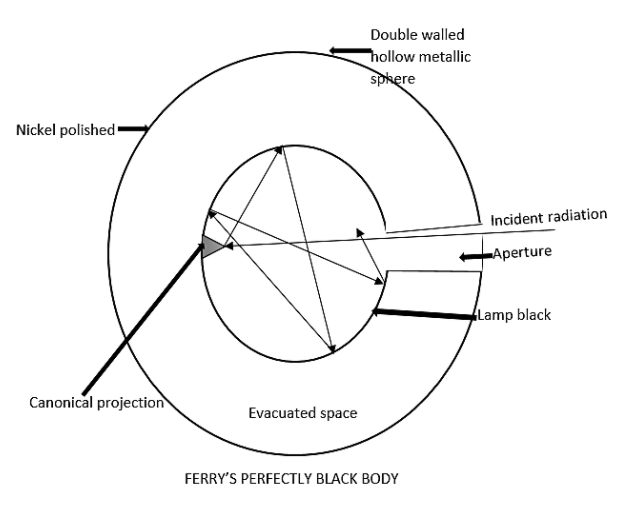
\includegraphics[keepaspectratio=true,scale=0.5]{blackbody.png}
\end{figure}


\newpage
\section{\underline{Energy distribution curve}}

Blackbody emits all radiations when maintained at constant temperature. The distribution of energy in a blackbody radiation for different wavelengths and at various temperatures was determined experimentally by Lummer and Pringshiem in 1899. A graph of intensity $E_{\lambda}$ and wavelength $\lambda$ was plotted at different temperatures. 
\begin{figure}[H]
	\centering
	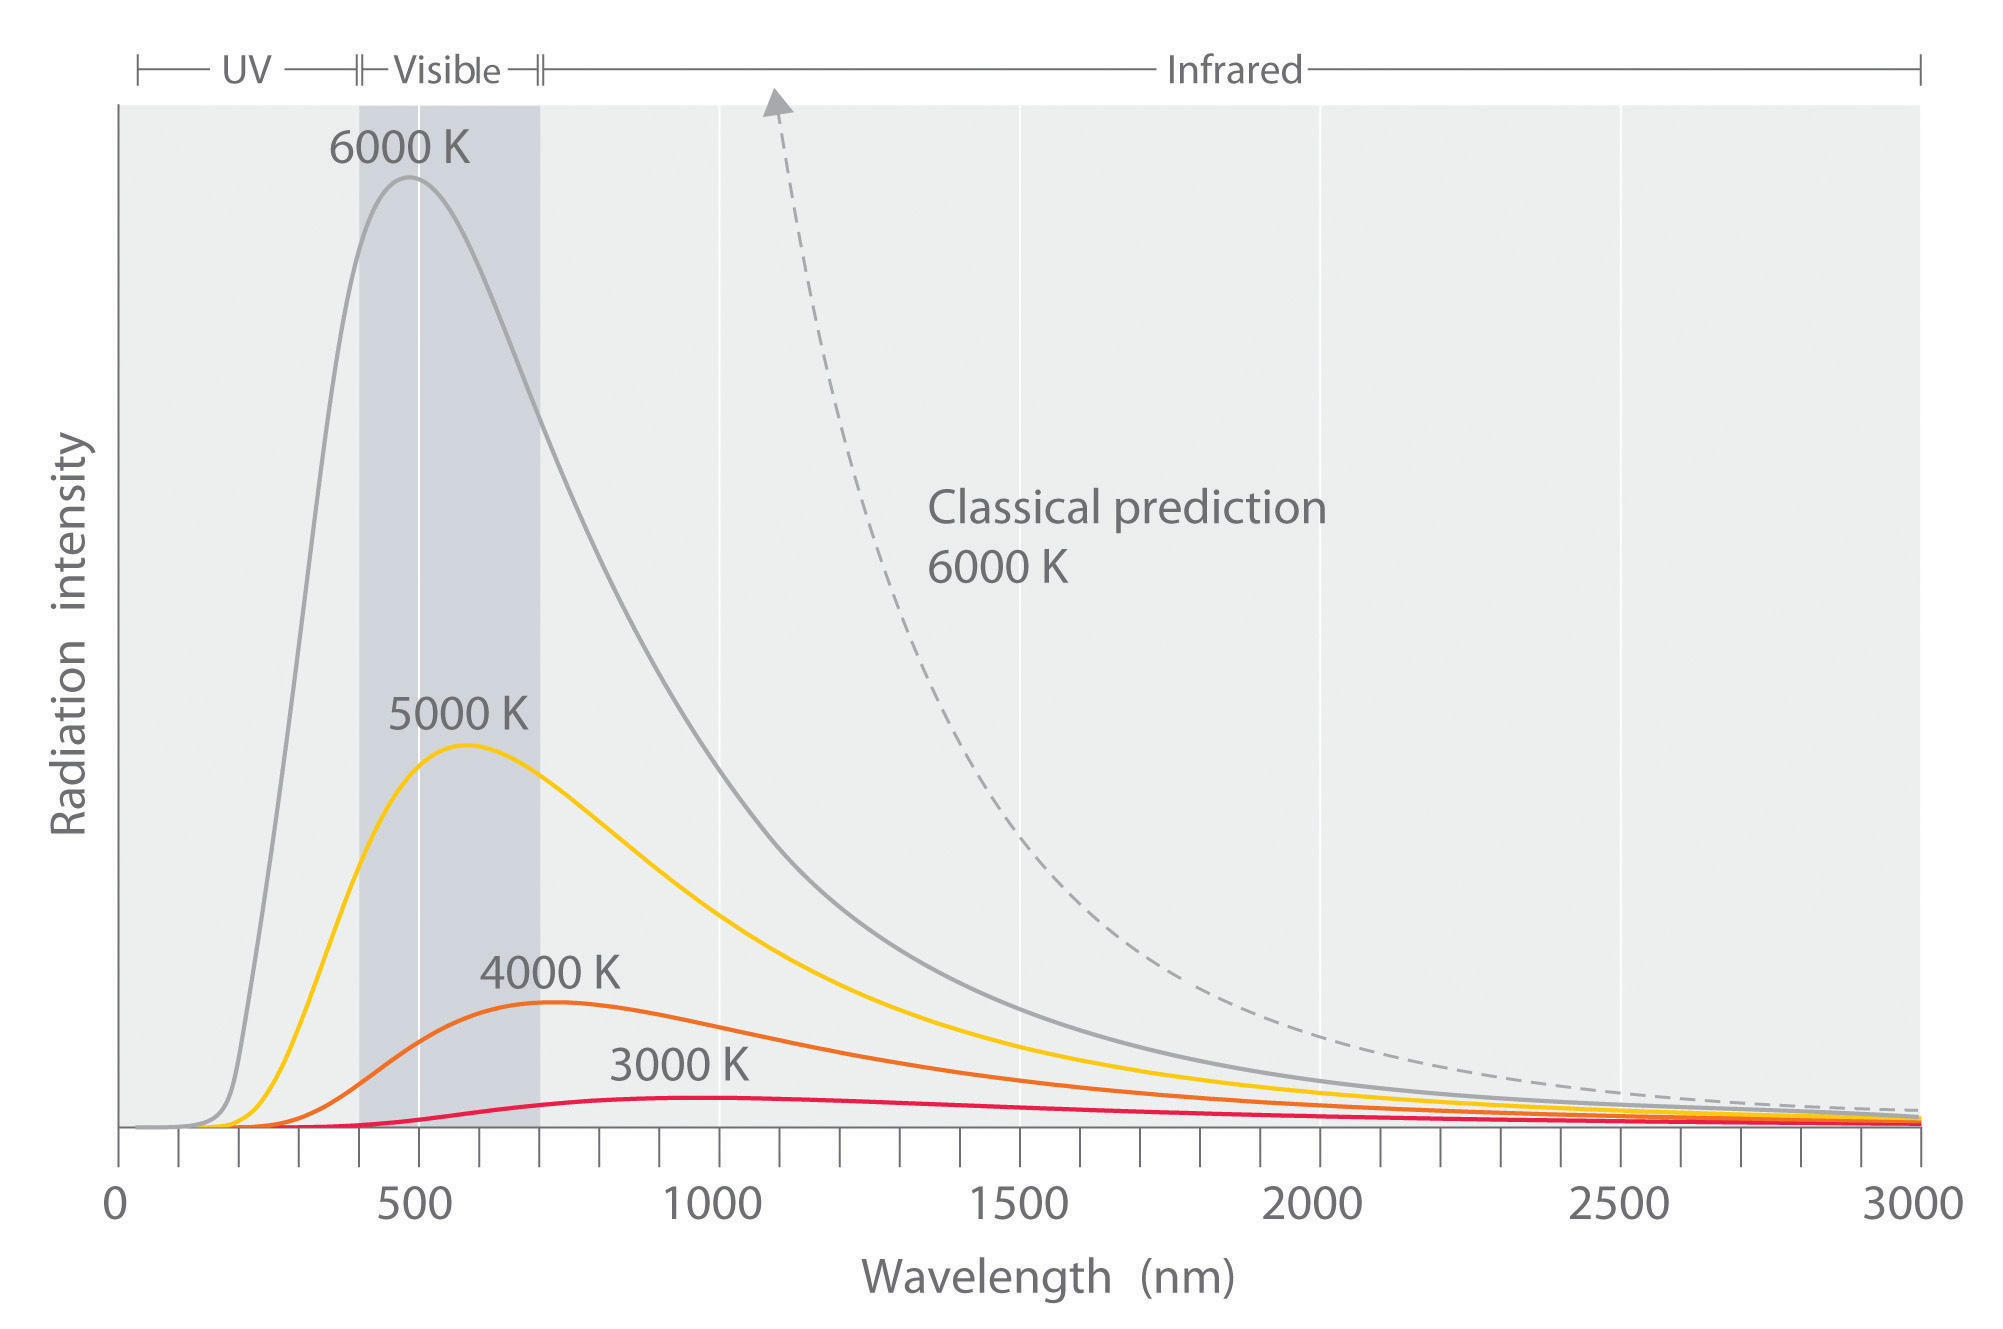
\includegraphics[keepaspectratio=true,scale=0.22]{blackbody_curve.jpg}
\end{figure}

\subsection{\textbf{Observations}}
\begin{enumerate}
    \item Blackbody emits all types of radiations ranging from lower wavelength to higher wavelength.
    \item The energy is not distributed uniformly among the wavelengths.
    \item At a given temperature the intensity of radiation increase with increase in wavelength and becomes maximum at a particular wavelength ($\lambda_{m}$). By farther increasing the wavelength, the intensity of radiation decreases.
    \item The wavelength ($\lambda_{m}$) corresponding to maximum intensity get shifted towards lower wavelengths with increase of temperature.
    \item Energy emitted due to all wavelengths increasing with increase in temperature.\\
    (This is in accordance with \textbf{Stefan-Boltzmann's law})
\end{enumerate}
\newpage
\section{\underline{Wien's distribution law}}
    \subsection{\textbf{Wien's displacement law}} \textit{"The wavelength $\lambda_{m}$ corresponding to maximum intensity of emission of blackbody radiation is inversely proportional to the absolute temperature $T$ of the body emitting radiation."}
    \begin{equation*}
        \lambda_{m} \propto \frac{1}{T}
    \end{equation*}
    or
    \begin{equation}
        \lambda_{m} = \frac{b}{T}
    \end{equation}
    where,  $b = 2.898 \times 10^{3} mK$.
This is called the \textbf{displacement law} because the maximum intensity of radiation emitted by a blackbody gets shifted towards shorter wavelength side with increase in temperature of the body.
    \subsection{\textbf{Fifth power law}}  \textit{"The maximum energy $E_{m}$ of the peak emission is directly proportional to the fifth power of absolute temperature of the blackbody."}
    \begin{equation*}
        E_{m} \propto T^{5}
    \end{equation*}
    or
    \begin{equation}
        E_{m} = (constant)T^{5}
    \end{equation}
Combining the two laws, the energy density of radiation in the wavelength range $\lambda$ and $\lambda+d\lambda$ as
    \begin{equation}
        E_{\lambda} = (constant)\lambda^{5} f(\lambda,T) 
    \end{equation}
This is called \textbf{Wien's distribution law}. It explains only the increasing part of the curve, in the shorter wavelength region but failed to explain the decreasing part of the curve, the higher wavelength region.

\section{\underline{Rayleigh-Jean's law}} 
Wien's distribution law failed in explaining the decreasing part of the energy distribution curve, Lord Rayleigh, therefore, sought to determine its form on the basis of classical ideas and was later developed by Jean. According to them the energy  density of the blackbody radiation within the wavelength range $\lambda$ and $\lambda+d\lambda$ is 
\begin{equation}
    E_{\lambda} = 8\pi kT\lambda^{-4}d\lambda
\end{equation}
This is called \textbf{Rayleigh-Jean's law} of energy distribution of blackbody radiation. This agrees well with the experimental results in the longer wavelength region nut fails in the shorter wavelength region.
\subsection{The Ultraviolet catastrophe}
According to the Rayleigh-Jean's law, the energy density is given by,
\begin{equation*}
    E_{\lambda} = 8\pi kT\lambda^{-4}d\lambda
\end{equation*}
The energy density of blackbody radiation will continuously increase with the decrease of wavelength an approaches infinity with the $\lambda \rightarrow 0 $. This shows that all the thermal energy in the universe will manifest itself in the form of short wavelengths. This is against to the experimental observations. This fatal objection to the Rayleigh-Jean's law at shorter wavelength is known as the \textbf{ultraviolet catastrophe}. The concept led classical physics to fail.
\newpage
\section{\underline{Planck's hypothesis and quantum theory}}
In order to explain the distribution of energy in the spectrum of blackbody over the entire range of wavelengths, Max Planck proposed a quantum theory of radiation in 1901. It is based on these following assumptions:
\begin{enumerate}
    \item The chamber which emits radiation is assumed to consists of large number of oscillators, each having its own natural frequency.
    \item These oscillators cannot emit or absorb energy continuously.
    \item Radiation is absorbed or emitted by oscillators in discrete packets of energy called  \textbf{quanta}. Energy of each quantum is $E = h\nu$, where $h = 6.626 \times 10^{-34} Js$ is called the \textbf{planck's constant} and $\nu$ is the frequency of the radiation emitted or absorbed. Thus, the energy of an oscillator may be $h\nu$, $2h\nu$, $3h\nu$ $\cdots$ or $nh\nu$, where $n$ is an integer.
    \\
    \textbf{The Planck's law of radiation.}
    \begin{Large}\begin{equation}
        E_{\lambda} d\lambda = \frac{8\pi hc}{\lambda^{5}} \left( \frac{1}{e^{\frac{hc} {kT \lambda} -1 } }  \right)d\lambda
    \end{equation}
    \end{Large}
\end{enumerate}
\end{document}


